\begin{flushright} {\tiny {\color{gray} dgfem2D.tex}} \end{flushright}
%~~~~~~~~~~~~~~~~~~~~~~~~~~~~~~~~~~~~~~~~~~~~~~~~~~~~~~~~~~~~~~~~~~~~~~~~~~~~~~~~~~~~~~~~~~~~~~~~~~

Let us start from the 2D steady state heat diffusion equation:
\begin{equation}
\vec{\nabla} \cdot k \vec{\nabla} T + H=0
\end{equation}
Just as in the 1D case this equation can be split in two separate first order differential equations:
\begin{equation}
\underbrace{-\vec{\nabla}\cdot \vec{q} + H=0}_{\text{ODE 1}} \qquad 
; \qquad \underbrace{\vec{q}=-k\vec{\nabla } T}_{\text{ODE 2}}
\end{equation}
Let $N^\uptheta_i$ be the temperature basis functions so that the temperature inside an element is given by
\begin{equation}
T_h (\vec{r}) = \sum_{i=1}^m N_i^\uptheta (\vec{r}) \; T_i = \vec{N^\uptheta}\cdot \vec{T}
\end{equation}
where $\vec{T}$ is a vector of length $m$, the number of nodes per element. 
Similarly we let the basis function for the heat flux be such that 
\begin{equation}
\qhx(\vec{r}) = \sum_{i=1}^m N_i^q (\vec r) \qix = \vec{N^q}\cdot \vec{\qx}
\end{equation}
\begin{equation}
\qhy(\vec{r}) = \sum_{i=1}^m N_i^q (\vec r) \qiy = \vec{N^q}\cdot \vec{\qy}
\end{equation}
where $\vec{\qx}$, $\vec{\qy}$ and $\vec{N}^q$ 
are vectors of length $m$ too. Implicitly if $m$ is the same for temperature and heat 
flux, then $N^\uptheta = N^q$.
Let us establish the weak forms of the 1st order ODEs. 

\paragraph{ODE 1} This results in:
\begin{eqnarray}
\int_\Omega {N^\uptheta_i} \vec{\nabla} \cdot \vec{q} \; dV = \int_\Omega {N^\uptheta_i} H \; dV
\label{eq:SSD2D}
\end{eqnarray}
Using the product rule $\vec{\nabla} \cdot ({N^\uptheta_i}\vec{q})={N^\uptheta_i}\vec{\nabla} \cdot \vec{q} 
+ \vec{\nabla}{N^\uptheta_i} \cdot \vec{q}$ then we can write
\[ 
{N^\uptheta_i}\vec{\nabla} \cdot \vec{q}=\vec{\nabla} \cdot ({N^\uptheta_i}\vec{q})- 
\vec{\nabla}{N^\uptheta_i} \cdot \vec{q}
\]
which we insert in Eq.~\eqref{eq:SSD2D} results in 
\begin{equation}
\int_{\Omega} \vec{\nabla} \cdot ({N^\uptheta_i} \vec{q}) \; dV - 
\int_{\Omega} \vec{\nabla} {N^\uptheta_i} \cdot \vec{q} \; dV = \int_{\Omega} {N^\uptheta_i} H \; dV
\label{eq:SSD2D1}
\end{equation}
Using the divergence theorem 
$\int_\Omega \vec{\nabla} \cdot \vec{F} \; d\Omega = \int_{d\Omega}(\vec{F} \cdot \vec{n}) \; dS$ 
 applied to Eq.~\eqref{eq:SSD2D1} leads to
\begin{equation}
\int_{d\Omega}{N^\uptheta_i} \vec{\hat{q}} \cdot \vec{n} \; dS  - 
\int_{\Omega} \vec{\nabla} {N^\uptheta_i} \cdot \vec{q} \; dV = 
\int_{\Omega} {N^\uptheta_i} H  \; dV
\end{equation}

Here $\vec{n}$ is the outward vector everywhere on the boundary. 
The exact solution $\vec{q}=(\qx,\qy)$ can be approximated with $\vec{q}_h$ in a  
finite element space, same for the approximation of the flux at the boundary $\hat{q}=\hat{q_h}$ 
which takes a special form in the context of the DG methods (as reflected by the presence of the hat).
We decompose the resulting equation in 3 terms $A$, $B$ and $C$:
\begin{equation}
\underbrace{ \int_{d\Omega}{N^\uptheta_i} \vec{\hat{q_h}} \cdot \vec{n} \; dS}_{A } - 
\underbrace{ \int_{\Omega} \vec{\nabla} {N^\uptheta_i} \cdot \vec{q_h} \; dV}_{B} = 
\underbrace{\int_{\Omega} {N^\uptheta_i} H  \;dV }_C
\label{eq:q2dss}
\end{equation}
%To make things very explicit, we can split the heat flux in its $x$ and $y$ component in the above equation:
%\begin{equation}
%\int_{d\Omega}  {N^\theta} (\hat{\qx} \nx + \hat{\qy} \ny) \; dS  -  
%\int_{\Omega} ( \partial_x N^\theta \qx   + 
%\partial_y N^\theta \qy ) \; dV = 
%\int_{\Omega} {N^\theta} H dV
%\label{eq:q2dss}
%\end{equation}
Note that terms $B$ and $C$ are explained in Section~\ref{ss:hte_diff}.
In all what follows blue symbols belong the the element under consideration 
and brown symbols belong to its neighbour(s).

\begin{center}
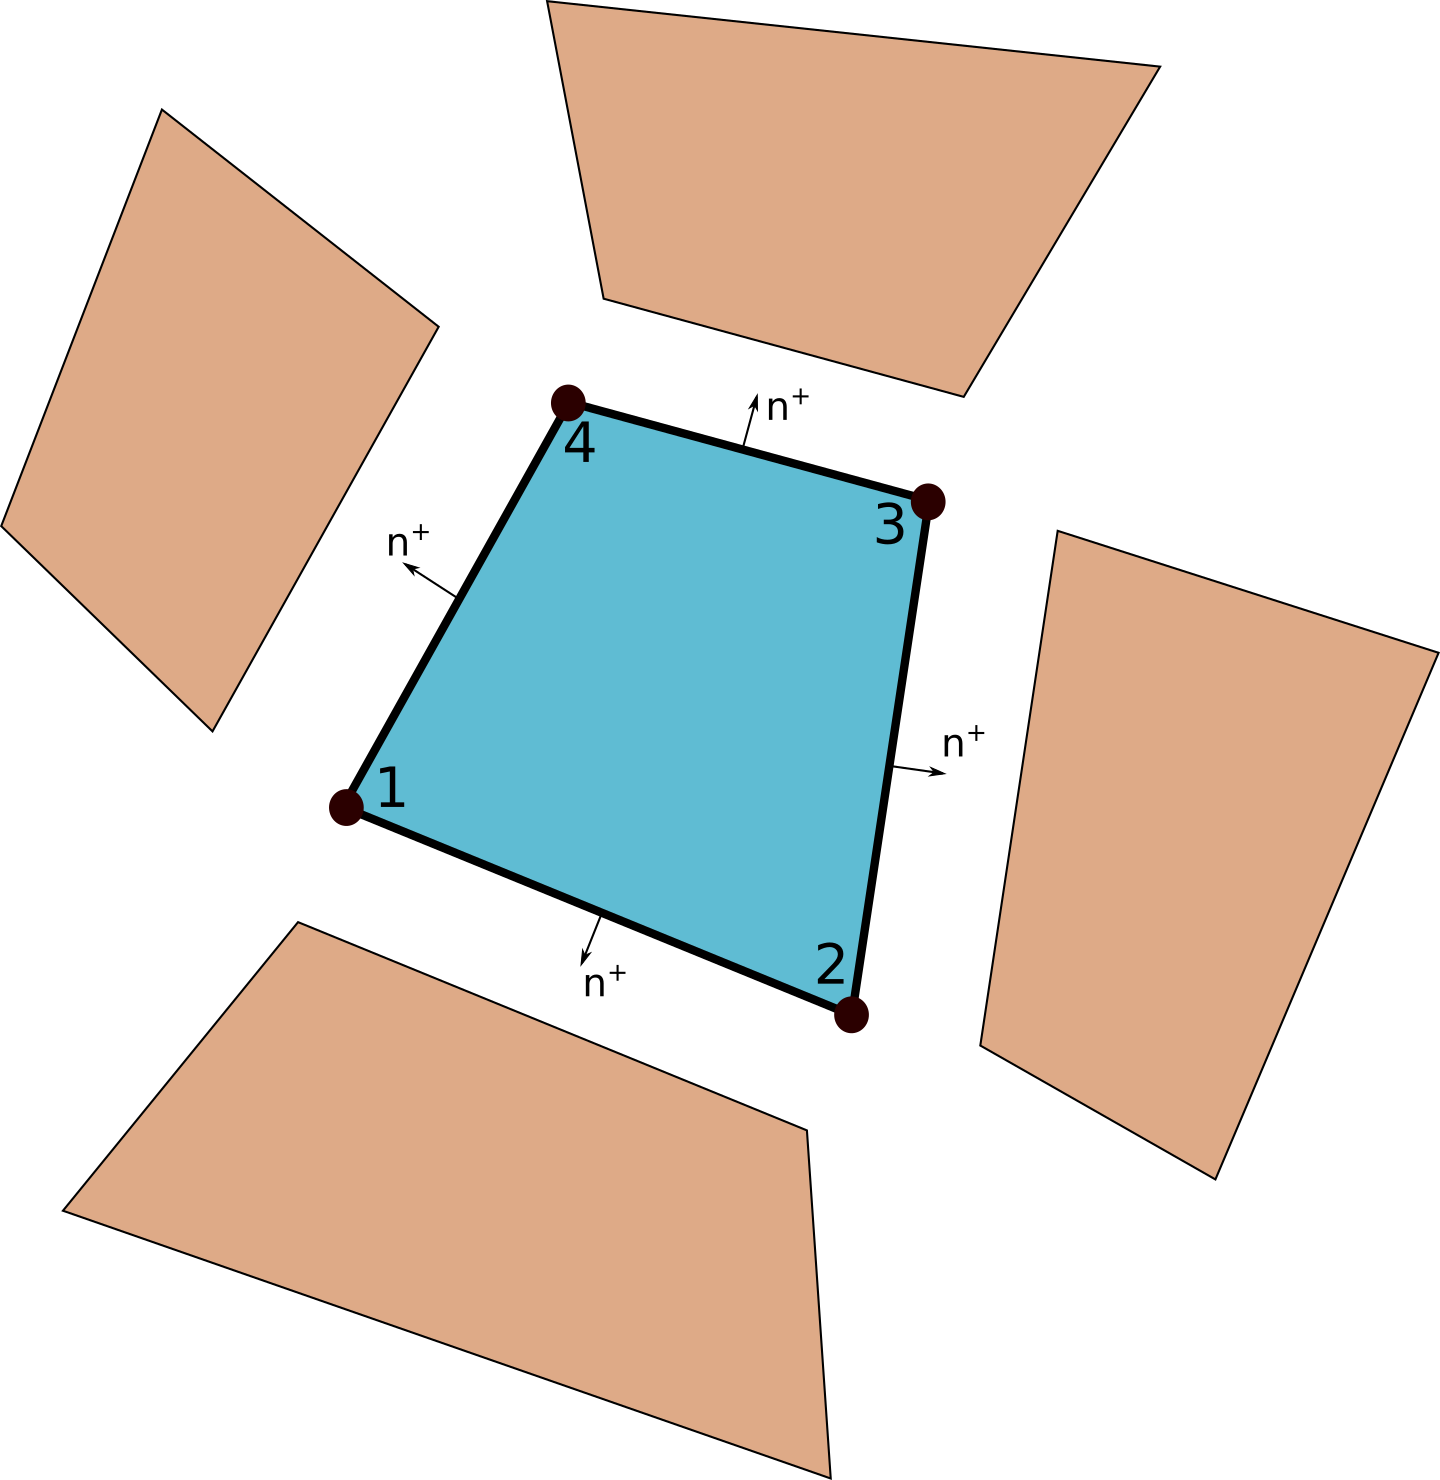
\includegraphics[width=7cm]{images/dgfem/dgelts}
\end{center}

%Here the blue color (before: $el$ superscript) indicates that it belongs to the element of interest and brown color (before: the $nb$ superscript) 
%denotes the values belonging to the neighbouring element. 
$\vec{n}^+$ indicates the outward vector at the boundary and $\vec{n}^-$ is 
the outward vector of the neighbouring element.

Let us turn to Li's book for useful definitions:
\begin{itemize}
\item
\underline{Definition of jump operators} The square brackets denote the jump operator:
\begin{eqnarray}
[\vec{q}_h] &=& \vec{\color{blue}q}_h \cdot \vec{n}^+ + \vec{\color{brown} q}_h \cdot \vec{n}^- 
\qquad \text{or} \qquad 
[\vec{q}_h]= (\vec{\color{blue}q}_h - \vec{\color{brown}q}_h) \cdot \vec{n}^+    \nn\\
\left[T_h\right] &=& \blueT_h \vec{n}^+ + {\brownT}_h \vec{n}^-  \qquad \text{or} \qquad 
[T_h]=(\blueT_h  - \brownT_h ) \; \vec{n}^+ 
\end{eqnarray}
%[q_{h,x}]=q_{h,x}^{el}n_x^+ + q_{h,x}^{nb}n_x^- \nn \\
%[q_{h,y}]=q_{h,y}^{el}n_y^+ + q_{h,y}^{nb}n_y^- \nn \\

Note that $[\vec{q}_h]$ is a scalar function which involves the
normal components only; while $[T_h]$ is a vector function. 

\item
\underline{Definition of average operators} The curly brackets indicate the average operator
\begin{eqnarray}
\{ \vec{q}_h \}&=&\frac{1}{2}(\vec{\color{blue}q}_h + \vec{\color{brown}q}_h)
\qquad \text{so} \quad 
\{\qhx\}=\frac{1}{2}(\blueqx_h + \brownqx_h) 
\qquad \text{and}
\qquad  \{\qhy\}=\frac{1}{2}(\blueqy_h + \brownqy_h) \nn \\
\{T_h\}&=&\frac{1}{2}(\blueT_h + \brownT_h) \nn 
\end{eqnarray}
Note that $\{ \vec{q}_h \}$ is a vector, while 
$\{T_h\}$ is a scalar.

\item
\underline{Definitions of fluxes} In the LDG method the boundary flux $\vec{\hat{q}}$ is defined as 
\[
\vec{\hat{q_h}} = \{ \vec{q_h} \} -{\cal{E}} [T_h]- \vec{\cal{C}}\;  [\vec{q_h}] 
\]
where ${\cal{E}}$ is a scalar (since $[T_h]$ is a vector)
and $\vec{\cal C}$ is a vector (since $[\vec{q}_h]$ is a scalar).
To be once again very explicit, the above equation writes as follows for a 
2D Cartesian space:
\begin{eqnarray}
\hat{\qhx} 
&=& \{\qhx\} -{\cal{E}} [T_h]_x- {\cal{C}}_x  [\vec{q}_h] \nn\\
&=& \frac{1}{2}(\blueqx_h + \brownqx_h)
-{\cal{E}} (\blueT_h {n}_x^+ + \brownT_h {n}_x^-)
-{\cal{C}}_x  
(\vec{\color{blue}q}_h \cdot \vec{n}^+ +\vec{\color{brown}q}_h \cdot \vec{n}^-) \label{flux2Da}\\
\hat{\qhy} 
&=& \{\qhy\} -{\cal{E}} [T_h]_y- {\cal{C}}_y  [\vec{q}_h] \nn\\
&=& \frac{1}{2}(\blueqy_h + \brownqy_h)  
-{\cal{E}}  (\blueT_h {n}_y^+ + \brownT_h {n}_y^-)
-{\cal{C}}_y  (\vec{\color{blue} q}_h \cdot \vec{n}^+ +\vec{\color{brown}q}_h \cdot \vec{n}^-) \label{flux2Db}
\end{eqnarray}

\begin{remark}
In the book the note under table 4.1 states that the $C_{ij}$ 
coefficients are constant matrices, which is quite misleading since some are actually scalars and others vectors.
\end{remark}

\end{itemize}


Filling Eqs.~\eqref{flux2Da} and \eqref{flux2Db} into $A$ of 
Eq.~\eqref{eq:q2dss} leads to
%(note that I have introduced the upperscript + on the normal components 
%because the integration is on the boundary of the element - does that make sense?)

\begin{eqnarray}
A&=& \int_{\partial\Omega} N^\uptheta_i \vec{\hat{q_h}} \cdot \vec{n} \; dS \nn\\ 
&=&
\int_{\partial\Omega} N^\uptheta_i \left[ \{ \vec{q_h} \} -{\cal{E}} [T_h]- \vec{\cal{C}}  [\vec{q_h}] \right] \cdot \vec{n}^+ \; dS  \nn\\
&=&
\int_{\partial\Omega}{N^\uptheta_i} \left[ \frac{1}{2}(\vec{\color{blue}q}_h + \vec{\color{brown}q}_h) 
-{\cal{E}} (\blueT_h \vec{n}^+ + \brownT_h \vec{n}^-)- \vec{\cal{C}}  [\vec{q_h}] \right] \cdot \vec{n}^+ \; dS  \nn\\
&=&
\int_{\partial\Omega}{N^\uptheta_i} \left[ \frac{1}{2}(\vec{\color{blue}q}_h + \vec{\color{brown}q}_h)\cdot\vec{n}^+ 
  -{\cal{E}} (\blueT_h \vec{n}^+ + \brownT_h \vec{n}^-) \cdot \vec{n}^+
- \vec{\cal{C}} \cdot \vec{n}^+ [\vec{q_h}] \right] \; dS  \nn\\
&=&
\int_{\partial\Omega}{N^\uptheta_i} \left[ \frac{1}{2}(\vec{\color{blue}q}_h + \vec{\color{brown}q}_h)\cdot\vec{n}^+  -{\cal{E}} (\blueT_h -\brownT_h ) 
- (\vec{\cal{C}} \cdot \vec{n}^+) 
(\vec{\color{blue}q}_h - \vec{\color{brown}q}_h) \cdot \vec{n}^+
\right] \; dS  \qquad \text{since} \quad  \vec{n}^+\!\cdot\!\vec{n}^+ =1 \quad  \vec{n}^+\!\cdot\!\vec{n}^- =-1 \nn\\
&=&
\int_{\partial\Omega}{N^\uptheta_i} \left[
\left(\frac{1}{2} - \vec{\cal{C}} \cdot \vec{n}^+ \right) \vec{\color{blue}q}_h\cdot\vec{n}^+
- {\cal{E}} \blueT_h
\right] \; dS 
+ 
\int_{\partial\Omega}{N^\uptheta_i} \left[
\left(\frac{1}{2} + \vec{\cal{C}} \cdot \vec{n}^+ \right)
\vec{\color{brown}q}_h \cdot\vec{n}^+
+ {\cal{E}} \brownT_h
\right] \; dS  \nn \\
&=&
\int_{\partial\Omega}{N^\uptheta_i} 
\left(\frac{1}{2} - \vec{\cal{C}} \cdot \vec{n}^+ \right) \vec{\color{blue}q}_h\cdot\vec{n}^+ \; dS 
- \int_{\partial\Omega}{N^\uptheta_i}  {\cal{E}} \blueT_h  \; dS 
+ 
\int_{\partial\Omega}{N^\uptheta_i} \left(\frac{1}{2} + \vec{\cal{C}} \cdot \vec{n}^+ \right)
\vec{\color{brown}q}_h \cdot\vec{n}^+   \; dS
+
\int_{\partial\Omega}{N^\uptheta_i}   {\cal{E}} \brownT_h   \; dS  \nn \\
&=& A_1 + A_2 + A_3 + A_4 
\end{eqnarray}
In order to simplify notations we choose $N^q=N^\uptheta=N$ and drop the $h$ subscripts.

\begin{eqnarray}
A_1 
&=& \int_{\partial\Omega}{N_i} \left(\frac{1}{2} - \vec{\cal{C}} \cdot \vec{n}^+ \right) \vec{\color{blue}q}\cdot\vec{n}^+ \; dS \nn \\
&=& \int_{\partial\Omega}{N_i} \left(\frac{1}{2} - \vec{\cal{C}} \cdot \vec{n}^+ \right) ({\color{blue}q}_x n^+_x  +   {\color{blue}q}_y {n}_y^+) \; dS \nn \\
&=& \int_{\partial\Omega}{N_i} \left(\frac{1}{2} - \vec{\cal{C}} \cdot \vec{n}^+ \right) {\color{blue}q}_x n^+_x   \; dS 
+ \int_{\partial\Omega}{N_i} \left(\frac{1}{2} - \vec{\cal{C}} \cdot \vec{n}^+ \right)  {\color{blue}q}_y {n}_y^+ \; dS \nn \\
\Rightarrow {\vec A}_1
&=& \left( \int_{\partial\Omega}  \left(\frac{1}{2} - \vec{\cal{C}} \cdot \vec{n}^+ \right) \vec{N}^T \vec{N} n^+_x  \; dS  \right) \cdot {\color{blue}\vec{\qx}}  
+ \left( \int_{\partial\Omega}  \left(\frac{1}{2} - \vec{\cal{C}} \cdot \vec{n}^+ \right) \vec{N}^T \vec{N} n^+_y  \; dS  \right) \cdot {\color{blue}\vec{\qy}}  \\
A_2 &=& - \int_{\partial\Omega}{N_i}  {\cal{E}} \blueT  \; dS \nn\\
\Rightarrow {\vec A}_2 &=& - \left( \int_{\partial\Omega}   {\cal{E}}   \vec{N}^T \vec{N} dS \right) \cdot \vec{\blueT} \\
A_3 
&=& \int_{\partial\Omega}{N^\uptheta_i} \left(\frac{1}{2} + \vec{\cal{C}} \cdot \vec{n}^+ \right)
 \vec{\color{brown}q} \cdot\vec{n}^+   \; dS \nn\\
&=& \int_{\partial\Omega}{N^\uptheta_i} \left(\frac{1}{2} + \vec{\cal{C}} \cdot \vec{n}^+ \right)
 ({\color{brown}q}_x {n}_x^+  +  {\color{brown}q}_y {n}_y^+       )  \; dS \nn\\
&=& 
\int_{\partial\Omega}{N^\uptheta_i} \left(\frac{1}{2} + \vec{\cal{C}} \cdot \vec{n}^+ \right)  {\color{brown}q}_x {n}_x^+    \; dS 
+ \int_{\partial\Omega}{N^\uptheta_i} \left(\frac{1}{2} + \vec{\cal{C}} \cdot \vec{n}^+ \right)   {\color{brown}q}_y {n}_y^+    \; dS \nn\\
\Rightarrow {\vec A}_3 &=&
  \left(\int_{\partial\Omega} \left(\frac{1}{2} + \vec{\cal{C}} \cdot \vec{n}^+ \right) \vec{N}^T \vec{N} {n}_x^+    \; dS \right) \cdot  {\color{brown}\vec{\qx}}
+ \left(\int_{\partial\Omega} \left(\frac{1}{2} + \vec{\cal{C}} \cdot \vec{n}^+ \right) \vec{N}^T \vec{N} {n}_y^+    \; dS \right) \cdot  {\color{brown}\vec{\qy}} \\
A_4 &=& \int_{\partial\Omega}{N_i}   {\cal{E}}  \brownT   \; dS  \nn\\
\Rightarrow {\vec A}_4 &=&  \left( \int_{\partial\Omega}   {\cal{E}}   \vec{N}^T \vec{N} dS \right) \cdot \vec{\brownT} \\ 
B 
&=& \int_{\Omega} \vec{\nabla} {N_i} \cdot \vec{\color{blue} q} \; dV  \nn \\
&=& \int_{\Omega} (\partial_x N_i {\color{blue}q}_x + \partial_y N_i {\color{blue}q}_y )   \; dV  \nn \\
&=& \int_{\Omega} \partial_x N_i {\color{blue}q}_x   \; dV   
 +  \int_{\Omega} \partial_y N_i {\color{blue}q}_y   \; dV  \nn \\
\Rightarrow {\vec B} &=& 
  \left(\int_{\Omega} \partial_x \vec{N}^T \vec{N}   \; dV \right)\cdot {\color{blue}\vec{\qx}}  
+ \left(\int_{\Omega} \partial_y \vec{N}^T \vec{N}   \; dV \right)\cdot {\color{blue}\vec{\qy}}  \\
C &=& \int_{\Omega} {N_i} H  \;dV \nn \\
\Rightarrow {\vec C} &=& \int_{\Omega} \vec{N}^T H  \;dV  
\end{eqnarray}


The expressions above find their equivalent in the book (NB stands for neighbour):
\begin{center}
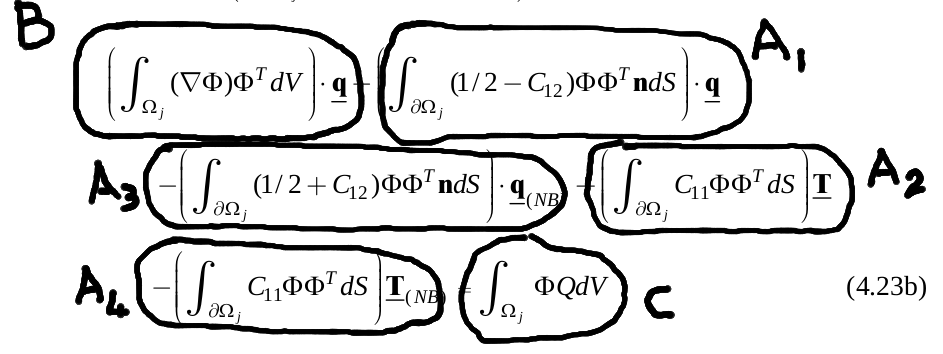
\includegraphics[width=10cm]{images/dgfem/li_01}\\
{\captionfont Note that in the book we have: $C_{12}={\bm C}_{12}\cdot {\bm n}^+ \rightarrow \vec{\cal C}\cdot\vec{n}^+$;
$C_{11} \rightarrow {\cal E}$}
\end{center}

\todo[inline]{check minus signs}




%---------------------------------------------------
\paragraph{ODE 2} Its weak form writes:
\[
\int_\Omega N_i^q (\vec{q} + k\vec{\nabla } T ) dV = 0
\]
or, (once again we drop the superscript on the basis functions and the $h$): 
\begin{eqnarray}
0 &=& \int_\Omega N_i \vec{q} \;  dV + \int_\Omega N_i k\vec{\nabla } T \; dV \nn\\
&=& \int_\Omega N_i \vec{q} \;  dV + \int_\Omega \vec\nabla (N_i k  T) \; dV 
- \int_\Omega \vec\nabla (k N_i) T \; dV
\end{eqnarray}
We then use $\int_\Omega \vec\nabla f \; dV = \int_{\partial\Omega} f \vec{dS}$
and as before the temperature on the edge integral should be $\hat{T}$:
\[
\int_\Omega N_i \vec{q} \;  dV + \int_{\partial\Omega}  k N_i \hat{T} \; \vec{n}^+  dS - \int_\Omega \vec\nabla (k N_i)   T \; dV = 0
\]
or, if decomposed in a 2D Cartesian axis system 
\begin{eqnarray}
0
%&=&\int_\Omega N_i \left( \qx + k  \frac{\partial T}{\partial x} \right) \; dV \nn\\
%&=&\int_\Omega N_i  \qx^h dV
%+ \int_\Omega N_i k  \frac{\partial T^h}{\partial x}  \; d\Omega \nn\\
&=& \underbrace{ \int_\Omega N_i  \qx \; dV }_{D}
+\underbrace{\int_{\partial\Omega} k N_i \hat{T} \; n^+_x \; dS}_{E}
-\underbrace{\int_\Omega \partial_x ( k N_i) \;  T \; dV}_{F} \qquad\qquad  (0=D+E-F)\nn\\
0
%&=&\int_\Omega N_i \left( \qy^h + k  \frac{\partial T^h}{\partial y} \right) \; dV \nn\\
%&=&\int_\Omega N_i  \qy^h dV
%+ \int_\Omega N_i k  \frac{\partial T^h}{\partial y}  \; d\Omega \nn\\
&=&\underbrace{\int_\Omega N_i  \qy \; dV}_G 
+\underbrace{\int_{\partial\Omega} k N_i  \hat{T} \; n^+_y \; dS }_{H}
-\underbrace{\int_\Omega \partial_y (k N_i) \;  T \; dV}_I \qquad\qquad  (0=G+H-I)
\end{eqnarray}
%Both can be summed together and creating the vector $\vec{N}=(N_i,N_i)= N_i(\vec{e}_x+\vec{e}_y)$ then we get 
%\[
%\int_\Omega \vec{N}_i \cdot \vec{q}^h dV 
%+\int_{\partial\Omega} k \hat{T} \vec{N}\cdot \vec{n}^+  dS
%-\int_\Omega \vec{\nabla}\cdot (\vec{N}_i k) \;  T \; dV 
%=0
%\]
which (aside from a minus sign coming from a different definition of the heat flux) is 'identical' to the book
(although the notations in the book are hella confusing):
\begin{center}
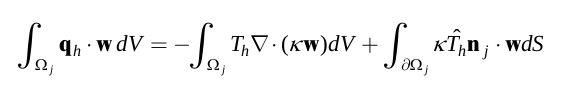
\includegraphics[width=8cm]{images/dgfem/li_02} (with $\kappa \rightarrow k$, ${\bm w}\rightarrow \vec{N}$)
\end{center}

\noindent 
The temperature flux $\hat{T}$ is chosen to be (table 4.1 in book):
\begin{eqnarray}
\hat{T}_h 
&=& \{ T_h \} + \vec{\cal C} [T_h] - {\cal F} [\vec{q}_h] \\
&=& \frac{1}{2}(\blueT_h + \brownT_h)   
+ \vec{\cal C} (\blueT_h \vec{n}^+ + {\brownT}_h \vec{n}^-) 
- {\cal F}   (\vec{\color{blue}q}_h \cdot \vec{n}^+ + \vec{\color{brown} q}_h \cdot \vec{n}^-) \\
&=& \frac{1}{2}(\blueT_h + \brownT_h)   
+  (\blueT_h  - \brownT_h ) \; \vec{\cal C}\cdot\vec{n}^+  
- {\cal F} (\vec{\color{blue}q}_h - \vec{\color{brown}q}_h) \cdot \vec{n}^+ \\
&=& \left( \frac{1}{2} + \vec{\cal C} \cdot \vec{n}^+ \right) \blueT_h 
+ \left( \frac{1}{2} - \vec{\cal C} \cdot \vec{n}^+ \right) \brownT_h 
- {\cal F} (\vec{\color{blue}q}_h - \vec{\color{brown}q}_h) \cdot \vec{n}^+ 
\end{eqnarray}



In what follows we assume $k$ to be constant within each element so that $\partial_x (k N_i)= k \partial_x N_i$.

\begin{eqnarray}
D &=& \int_\Omega N_i  \qx\;  dV 
\qquad \Rightarrow \qquad  \vec{D} = \left( \int_\Omega \vec{N}^T \vec{N} dV \right) \cdot {\color{blue}\vec{\qx}} \\ 
F &=& \int_\Omega k \partial_x N_i \;  T \; dV 
\qquad \Rightarrow \qquad \vec{F} = \left( \int_\Omega k \partial_x \vec{N}^T \vec{N} \; dV \right) \cdot \vec{\color{blue} T} \\
G &=&  \int_\Omega N_i  \qy^h \; dV
\qquad \Rightarrow \qquad \vec{G} = \left( \int_\Omega \vec{N}^T \vec{N} dV \right) \cdot {\color{blue}\vec{\qy}} \\ 
I &=&  \int_\Omega k \partial_y N_i \;  T \; dV 
\qquad \Rightarrow \qquad \vec{I} = \left( \int_\Omega k \partial_y \vec{N}^T \vec{N} \; dV \right) \cdot \vec{\color{blue} T} \\
E &=&  \int_{\partial\Omega} k N_i \hat{T} \; n^+_x dS \nn\\
 &=&  
\int_{\partial\Omega} k N_i 
\left[  \left( \frac{1}{2} + \vec{\cal C} \cdot \vec{n}^+ \right) \blueT_h 
+ \left( \frac{1}{2} - \vec{\cal C} \cdot \vec{n}^+ \right) \brownT_h 
- {\cal F} (\vec{\color{blue}q}_h - \vec{\color{brown}q}_h) \cdot \vec{n}^+ 
\right] n^+_x dS \nn\\
 &=&  
\int_{\partial\Omega} k N_i \left( \frac{1}{2} + \vec{\cal C} \cdot \vec{n}^+ \right) \blueT_h  n^+_x dS 
+\int_{\partial\Omega} k N_i \left( \frac{1}{2} - \vec{\cal C} \cdot \vec{n}^+ \right) \brownT_h   n^+_x dS \nn\\
&&-
\int_{\partial\Omega} k N_i  {\cal F} (\vec{\color{blue}q}_h \cdot \vec{n}^+ )  n^+_x dS 
+
\int_{\partial\Omega} k N_i  {\cal F} (\vec{\color{brown}q}_h \cdot \vec{n}^+ )  n^+_x dS \nn\\
&=& E_1  + E_2 + E_3 + E_4 \nn\\
H &=& 
\int_{\partial\Omega} k N_i  \hat{T} \; n^+_y dS \nn\\
&=& H_1+H_2+H_3+H_4
\end{eqnarray}

Then 
\begin{eqnarray}
E_1 &=&
\int_{\partial\Omega} k N_i \left( \frac{1}{2} + \vec{\cal C} \cdot \vec{n}^+ \right) \blueT_h  n^+_x dS 
\qquad \Rightarrow \qquad
\left(\int_{\partial\Omega} k \left( \frac{1}{2} + \vec{\cal C} \cdot \vec{n}^+ \right) {N}^T \vec{N} n^+_x dS \right)\cdot \vec{\color{blue}T} \nn\\
E_2 &=& 
\int_{\partial\Omega} k N_i \left( \frac{1}{2} - \vec{\cal C} \cdot \vec{n}^+ \right) \brownT_h   n^+_x dS
\qquad \Rightarrow \qquad
\left(\int_{\partial\Omega} k \left( \frac{1}{2} - \vec{\cal C} \cdot \vec{n}^+ \right) {N}^T \vec{N} n^+_x dS \right)\cdot \vec{\color{brown}T} \nn\\
E_3 
&=& -\int_{\partial\Omega} k N_i  {\cal F} (\vec{\color{blue}q}_h \cdot \vec{n}^+ )  n^+_x dS \nn\\ 
&=& -\int_{\partial\Omega} k N_i  {\cal F} ({\color{blue}q}_x {n}^+_x + {\color{blue}q}_y {n}^+_y )  n^+_x dS \nn\\ 
&=& -\int_{\partial\Omega} k N_i  {\cal F} {\color{blue}q}_x {n}^+_x   n^+_x dS 
   -\int_{\partial\Omega} k N_i  {\cal F} {\color{blue}q}_y {n}^+_y   n^+_x dS \nn\\
&\Rightarrow&  
 -\left(\int_{\partial\Omega} k \vec{N}^T\vec{N}  {\cal F} {n}^+_x   n^+_x dS \right)\cdot \vec{\blueqx} 
-\left(\int_{\partial\Omega} k \vec{N}^T\vec{N}  {\cal F} {n}^+_y   n^+_x dS \right)\cdot \vec{\blueqy} \nn\\
E_4 
&=& \int_{\partial\Omega} k N_i  {\cal F} (\vec{\color{brown}q}_h \cdot \vec{n}^+ )  n^+_x dS \nn\\
&=& \int_{\partial\Omega} k N_i  {\cal F} ({\color{brown}q}_x  {n}^+_x + {\color{brown}q}_y  {n}^+_y )  n^+_x dS \nn\\
&=& \int_{\partial\Omega} k N_i  {\cal F} {\color{brown}q}_x  {n}^+_x   n^+_x dS 
  + \int_{\partial\Omega} k N_i  {\cal F} {\color{brown}q}_y  {n}^+_y   n^+_x dS \nn\\
&\Rightarrow&  
 \left(\int_{\partial\Omega} k \vec{N}^T\vec{N}  {\cal F} {n}^+_x   n^+_x dS \right)\cdot \vec{\brownqx} 
+\left(\int_{\partial\Omega} k \vec{N}^T\vec{N}  {\cal F} {n}^+_y   n^+_x dS \right)\cdot \vec{\brownqy} 
\end{eqnarray}

The $H_i$ terms are so similar to the $E_i$ terms that there is not need to write them out explicitely.


\begin{landscape}

\noindent We have seen that ODE \#2 and \#1 write
\begin{eqnarray}
D+E-F = D+E_1+E_2+E_3+E_4-F &=&0\\
G+H-I = G+H_1+H_2+H_3+H_4-I &=&0\\
A-B = A_1 + A_2 + A_3 + A_4 - B &=& \vec{C}
\end{eqnarray}

so that 
\begin{eqnarray}
\left( \int_\Omega \vec{N}^T \vec{N} dV \right) \cdot {\color{blue}\vec{\qx}} 
+ \left(\int_{\partial\Omega} k \left( \frac{1}{2} + \vec{\cal C} \cdot \vec{n}^+ \right) {N}^T \vec{N} n^+_x dS \right)\cdot \vec{\color{blue}T} 
+ \left(\int_{\partial\Omega} k \left( \frac{1}{2} - \vec{\cal C} \cdot \vec{n}^+ \right) {N}^T \vec{N} n^+_x dS \right)\cdot \vec{\color{brown}T} && \nn\\
-\left(\int_{\partial\Omega} k \vec{N}^T\vec{N}  {\cal F} {n}^+_x   n^+_x dS \right)\cdot \vec{\blueqx} 
-\left(\int_{\partial\Omega} k \vec{N}^T\vec{N}  {\cal F} {n}^+_y   n^+_x dS \right)\cdot \vec{\blueqy} 
+ \left(\int_{\partial\Omega} k \vec{N}^T\vec{N}  {\cal F} {n}^+_x   n^+_x dS \right)\cdot \vec{\brownqx} 
+\left(\int_{\partial\Omega} k \vec{N}^T\vec{N}  {\cal F} {n}^+_y   n^+_x dS \right)\cdot \vec{\brownqy} 
- \left( \int_\Omega k \partial_x \vec{N}^T \vec{N} \; dV \right) \cdot \vec{\color{blue} T} &=& \vec{0} 
\nn\\
\nn\\
\left( \int_\Omega \vec{N}^T \vec{N} dV \right) \cdot {\color{blue}\vec{\qy}} 
+ \left(\int_{\partial\Omega} k \left( \frac{1}{2} + \vec{\cal C} \cdot \vec{n}^+ \right) {N}^T \vec{N} n^+_y dS \right)\cdot \vec{\color{blue}T} 
+ \left(\int_{\partial\Omega} k \left( \frac{1}{2} - \vec{\cal C} \cdot \vec{n}^+ \right) {N}^T \vec{N} n^+_y dS \right)\cdot \vec{\color{brown}T} && \nn\\
-\left(\int_{\partial\Omega} k \vec{N}^T\vec{N}  {\cal F} {n}^+_x   n^+_y dS \right)\cdot \vec{\blueqx} 
-\left(\int_{\partial\Omega} k \vec{N}^T\vec{N}  {\cal F} {n}^+_y   n^+_y dS \right)\cdot \vec{\blueqy} 
+ \left(\int_{\partial\Omega} k \vec{N}^T\vec{N}  {\cal F} {n}^+_x   n^+_y dS \right)\cdot \vec{\brownqx} 
+\left(\int_{\partial\Omega} k \vec{N}^T\vec{N}  {\cal F} {n}^+_y   n^+_y dS \right)\cdot \vec{\brownqy} 
- \left( \int_\Omega k \partial_y \vec{N}^T \vec{N} \; dV \right) \cdot \vec{\color{blue} T} &=& \vec{0} 
\nn \\
\nn \\
 \left( \int_{\partial\Omega}  \left(\frac{1}{2} - \vec{\cal{C}} \cdot \vec{n}^+ \right) \vec{N}^T \vec{N} n^+_x  \; dS  \right) \cdot {\color{blue}\vec{\qx}}  
+ \left( \int_{\partial\Omega}  \left(\frac{1}{2} - \vec{\cal{C}} \cdot \vec{n}^+ \right) \vec{N}^T \vec{N} n^+_y  \; dS  \right) \cdot {\color{blue}\vec{\qy}}  
 - \left( \int_{\partial\Omega}   {\cal{E}}   \vec{N}^T \vec{N} dS \right) \cdot \vec{\blueT}  && \nn\\
+  \left(\int_{\partial\Omega} \left(\frac{1}{2} + \vec{\cal{C}} \cdot \vec{n}^+ \right) \vec{N}^T \vec{N} {n}_x^+    \; dS \right) \cdot  {\color{brown}\vec{\qx}}
+ \left(\int_{\partial\Omega} \left(\frac{1}{2} + \vec{\cal{C}} \cdot \vec{n}^+ \right) \vec{N}^T \vec{N} {n}_y^+    \; dS \right) \cdot  {\color{brown}\vec{\qy}} 
+  \left( \int_{\partial\Omega}   {\cal{E}}   \vec{N}^T \vec{N} dS \right) \cdot \vec{\brownT} 
- \left(\int_{\Omega} \partial_x \vec{N}^T \vec{N}   \; dV \right)\cdot {\color{blue}\vec{\qx}}  
- \left(\int_{\Omega} \partial_y \vec{N}^T \vec{N}   \; dV \right)\cdot {\color{blue}\vec{\qy}}  
&=&
\int_{\Omega} \vec{N}^T H  \;dV \nn 
\end{eqnarray}










\begin{footnotesize}
\[
\left[
\underbrace{
\left(
\begin{array}{ccc}
\int_\Omega \vec{N}^T \vec{N} dV & 0 & -\int_\Omega k \partial_x \vec{N}^T \vec{N} \; dV \\ \\
0 & \int_\Omega \vec{N}^T \vec{N} dV & -\int_\Omega k \partial_y \vec{N}^T \vec{N} \; dV \\ \\
- \int_{\Omega} \partial_x \vec{N}^T \vec{N}   \; dV & 
- \int_{\Omega} \partial_y \vec{N}^T \vec{N}   \; dV & 0 
\end{array}
\right)}_{{\cal A}_\Omega}
+
\underbrace{
\left(
\begin{array}{ccc}
-\int_{\partial\Omega} k \vec{N}^T\vec{N}  {\cal F} {n}^+_x   n^+_x dS &  
-\int_{\partial\Omega} k \vec{N}^T\vec{N}  {\cal F} {n}^+_y   n^+_x dS & 
\int_{\partial\Omega} k \left( \frac{1}{2} + \vec{\cal C} \cdot \vec{n}^+ \right) {N}^T \vec{N} n^+_x dS 
\\ \\ 
-\int_{\partial\Omega} k \vec{N}^T\vec{N}  {\cal F} {n}^+_x   n^+_y dS & 
-\int_{\partial\Omega} k \vec{N}^T\vec{N}  {\cal F} {n}^+_y   n^+_y dS &
\int_{\partial\Omega} k \left( \frac{1}{2} + \vec{\cal C} \cdot \vec{n}^+ \right) {N}^T \vec{N} n^+_y dS 
\\ \\
 \int_{\partial\Omega}  \left(\frac{1}{2} - \vec{\cal{C}} \cdot \vec{n}^+ \right) \vec{N}^T \vec{N} n^+_x  \; dS & 
 \int_{\partial\Omega}  \left(\frac{1}{2} - \vec{\cal{C}} \cdot \vec{n}^+ \right) \vec{N}^T \vec{N} n^+_y  \; dS &
-  \int_{\partial\Omega}   {\cal{E}}   \vec{N}^T \vec{N} dS 
\end{array}
\right)}_{{\cal A}_{\partial\Omega}}
\right]
\cdot
\left(
\begin{array}{c} 
\vec{\blueqx} \\ \\ \vec{\blueqy} \\ \\ \vec{\color{blue}T} 
\end{array}
\right)
\]
\[
=
\left(
\begin{array}{ccc}
-\int_{\partial\Omega} k \vec{N}^T\vec{N}  {\cal F} {n}^+_x   n^+_x dS & 
-\int_{\partial\Omega} k \vec{N}^T\vec{N}  {\cal F} {n}^+_y   n^+_x dS & 
-\int_{\partial\Omega} k \left( \frac{1}{2} - \vec{\cal C} \cdot \vec{n}^+ \right) {N}^T \vec{N} n^+_x dS 
\\ \\
-\int_{\partial\Omega} k \vec{N}^T\vec{N}  {\cal F} {n}^+_x   n^+_y dS &
-\int_{\partial\Omega} k \vec{N}^T\vec{N}  {\cal F} {n}^+_y   n^+_y dS & 
-\int_{\partial\Omega} k \left( \frac{1}{2} - \vec{\cal C} \cdot \vec{n}^+ \right) {N}^T \vec{N} n^+_y dS 
\\ \\
-\int_{\partial\Omega} \left(\frac{1}{2} + \vec{\cal{C}} \cdot \vec{n}^+ \right) \vec{N}^T \vec{N} {n}_x^+    \; dS & 
-\int_{\partial\Omega} \left(\frac{1}{2} + \vec{\cal{C}} \cdot \vec{n}^+ \right) \vec{N}^T \vec{N} {n}_y^+    \; dS &
-\int_{\partial\Omega}   {\cal{E}}   \vec{N}^T \vec{N} dS 
\end{array}
\right)
\cdot 
\left( \begin{array}{c}  \vec{\brownqx} \\ \\ \vec{\brownqy} \\ \\ \vec{\color{brown}T}  \end{array} \right)
+
\left( \begin{array}{c} 0 \\ \\ 0  \\ \\ \int_{\Omega} \vec{N}^T H  \;dV   \end{array} \right)
\]
\end{footnotesize}

\begin{footnotesize}
\[
\left[
\underbrace{
\left(
\begin{array}{ccc}
\int_\Omega \vec{N}^T \vec{N} dV & 0 & -\int_\Omega k \partial_x \vec{N}^T \vec{N} \; dV \\ \\
0 & \int_\Omega \vec{N}^T \vec{N} dV & -\int_\Omega k \partial_y \vec{N}^T \vec{N} \; dV \\ \\
- \int_{\Omega} \partial_x \vec{N}^T \vec{N}   \; dV & 
- \int_{\Omega} \partial_y \vec{N}^T \vec{N}   \; dV & 0 
\end{array}
\right)}_{{\cal A}_\Omega}
+
\underbrace{
\sum_{i=1}^{nedges}
\left(
\begin{array}{ccc}
-\int_{\partial\Omega_i} k \vec{N}^T\vec{N}  {\cal F} {n}^+_x   n^+_x dS &  
-\int_{\partial\Omega_i} k \vec{N}^T\vec{N}  {\cal F} {n}^+_y   n^+_x dS & 
 \int_{\partial\Omega_i} k \left( \frac{1}{2} + \vec{\cal C} \cdot \vec{n}^+ \right) {N}^T \vec{N} n^+_x dS 
\\ \\ 
-\int_{\partial\Omega_i} k \vec{N}^T\vec{N}  {\cal F} {n}^+_x   n^+_y dS & 
-\int_{\partial\Omega_i} k \vec{N}^T\vec{N}  {\cal F} {n}^+_y   n^+_y dS &
 \int_{\partial\Omega_i} k \left( \frac{1}{2} + \vec{\cal C} \cdot \vec{n}^+ \right) {N}^T \vec{N} n^+_y dS 
\\ \\
 \int_{\partial\Omega_i}  \left(\frac{1}{2} - \vec{\cal{C}} \cdot \vec{n}^+ \right) \vec{N}^T \vec{N} n^+_x  \; dS & 
 \int_{\partial\Omega_i}  \left(\frac{1}{2} - \vec{\cal{C}} \cdot \vec{n}^+ \right) \vec{N}^T \vec{N} n^+_y  \; dS &
-\int_{\partial\Omega_i}   {\cal{E}}   \vec{N}^T \vec{N} dS 
\end{array}
\right)}_{{\cal A}_{\partial\Omega}}
\right]
\cdot
\left(
\begin{array}{c} 
\vec{\blueqx} \\ \\ \vec{\blueqy} \\ \\ \vec{\color{blue}T} 
\end{array}
\right)
\]
\[
=
\sum_{i=1}^{nedges}
\left(
\begin{array}{ccc}
-\int_{\partial\Omega_i} k \vec{N}^T\vec{N}  {\cal F} {n}^+_x   n^+_x dS & 
-\int_{\partial\Omega_i} k \vec{N}^T\vec{N}  {\cal F} {n}^+_y   n^+_x dS & 
-\int_{\partial\Omega_i} k \left( \frac{1}{2} - \vec{\cal C} \cdot \vec{n}^+ \right) {N}^T \vec{N} n^+_x dS 
\\ \\
-\int_{\partial\Omega_i} k \vec{N}^T\vec{N}  {\cal F} {n}^+_x   n^+_y dS &
-\int_{\partial\Omega_i} k \vec{N}^T\vec{N}  {\cal F} {n}^+_y   n^+_y dS & 
-\int_{\partial\Omega_i} k \left( \frac{1}{2} - \vec{\cal C} \cdot \vec{n}^+ \right) {N}^T \vec{N} n^+_y dS 
\\ \\
-\int_{\partial\Omega_i} \left(\frac{1}{2} + \vec{\cal{C}} \cdot \vec{n}^+ \right) \vec{N}^T \vec{N} {n}_x^+    \; dS & 
-\int_{\partial\Omega_i} \left(\frac{1}{2} + \vec{\cal{C}} \cdot \vec{n}^+ \right) \vec{N}^T \vec{N} {n}_y^+    \; dS &
-\int_{\partial\Omega_i}   {\cal{E}}   \vec{N}^T \vec{N} dS 
\end{array}
\right)
\cdot 
\left( \begin{array}{c}  \vec{\brownqx} \\ \\ \vec{\brownqy} \\ \\ \vec{\color{brown}T}  \end{array} \right)_i
+
\left( \begin{array}{c} 0 \\ \\ 0  \\ \\ \int_{\Omega} \vec{N}^T H  \;dV   \end{array} \right)
\]
\end{footnotesize}


\[
\left[
\left(
\begin{array}{ccc}
{\bm E} & {\bm 0} & {\bm H}_x \\
{\bm 0} & {\bm E} & {\bm H}_y \\
{\bm J}_x & {\bm J}_y & {\bm 0}
\end{array}
\right)
+
\sum_{i=1}^{nedges}
\left(
\begin{array}{ccc}
{\bm E}_{xx,i} & {\bm E}_{xy,i} & {\bm H}_{x,i} \\
{\bm E}_{yx,i} & {\bm E}_{yy,i} & {\bm H}_{y,i} \\
{\bm J}_{x,i} & {\bm J}_{y,i} & {\bm G}_{T,i}
\end{array}
\right)
\right]
\cdot
\left(
\begin{array}{c} 
\vec{\blueqx} \\  \vec{\blueqy} \\  \vec{\color{blue}T} 
\end{array}
\right)
=
\]




which is identical to the equation 4.24 in Li's book (if the terms related to the third dimension are disregarded):
\begin{center}
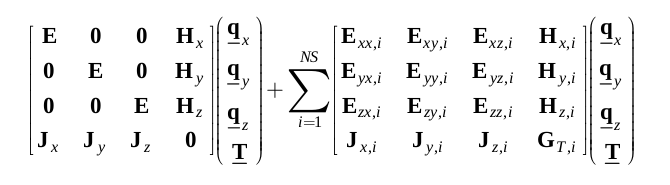
\includegraphics[width=8cm]{images/dgfem/li_04}+
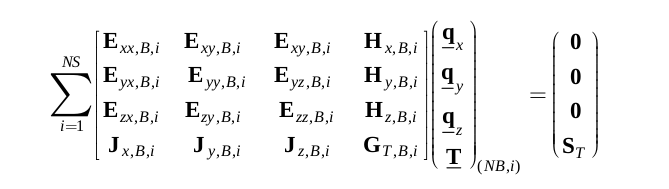
\includegraphics[width=8cm]{images/dgfem/li_05}
\end{center}
\end{landscape}

\begin{footnotesize}
\begin{eqnarray}
{\bm E} &=& \int_\Omega \vec{N}^T \vec{N} dV \\
{\bm H}_x &=&   -\int_\Omega k \partial_x \vec{N}^T \vec{N} \; dV     \\ 
{\bm H}_y &=&   -\int_\Omega k \partial_y \vec{N}^T \vec{N} \; dV     \\ 
{\bm J}_x &=&   -\int_\Omega  \partial_x \vec{N}^T \vec{N} \; dV     \\ 
{\bm J}_y &=&   -\int_\Omega  \partial_y \vec{N}^T \vec{N} \; dV     \\ 
{\bm E}_{xx,i} &=&   -\int_{\partial\Omega_i} k \vec{N}^T\vec{N}  {\cal F} {n}^+_x   n^+_x dS  \\
{\bm E}_{xy,i} &=&   -\int_{\partial\Omega_i} k \vec{N}^T\vec{N}  {\cal F} {n}^+_y   n^+_x dS  \\
{\bm E}_{yx,i} &=&    -\int_{\partial\Omega_i} k \vec{N}^T\vec{N}  {\cal F} {n}^+_x   n^+_y dS  \\
{\bm E}_{yy,i} &=&    -\int_{\partial\Omega_i} k \vec{N}^T\vec{N}  {\cal F} {n}^+_y   n^+_y dS  \\
{\bm H}_{x,i} &=&       \int_{\partial\Omega_i} k \left( \frac{1}{2} + \vec{\cal C} \cdot \vec{n}^+ \right) {N}^T \vec{N} n^+_x dS \\
{\bm H}_{y,i} &=&      \int_{\partial\Omega_i} k \left( \frac{1}{2} + \vec{\cal C} \cdot \vec{n}^+ \right) {N}^T \vec{N} n^+_y dS \\
{\bm J}_{x,i} &=&    \int_{\partial\Omega_i}  \left(\frac{1}{2} - \vec{\cal{C}} \cdot \vec{n}^+ \right) \vec{N}^T \vec{N} n^+_x  \; dS  \\
{\bm J}_{y,i} &=&    \int_{\partial\Omega_i}  \left(\frac{1}{2} - \vec{\cal{C}} \cdot \vec{n}^+ \right) \vec{N}^T \vec{N} n^+_y  \; dS  \\
{\bm G}_{T,i} &=&   -\int_{\partial\Omega_i}   {\cal{E}}   \vec{N}^T \vec{N} dS  \\
{\bm E}_{xx,B,i} &=&     -\int_{\partial\Omega_i} k \vec{N}^T\vec{N}  {\cal F} {n}^+_x   n^+_x dS \\
{\bm E}_{xy,B,i} &=&     -\int_{\partial\Omega_i} k \vec{N}^T\vec{N}  {\cal F} {n}^+_y   n^+_x dS \\
{\bm E}_{yx,B,i} &=&      -\int_{\partial\Omega_i} k \vec{N}^T\vec{N}  {\cal F} {n}^+_x   n^+_y dS \\
{\bm E}_{yy,B,i} &=&      -\int_{\partial\Omega_i} k \vec{N}^T\vec{N}  {\cal F} {n}^+_y   n^+_y dS \\
{\bm H}_{x,B,i} &=&     -\int_{\partial\Omega_i} k \left( \frac{1}{2} - \vec{\cal C} \cdot \vec{n}^+ \right) {N}^T \vec{N} n^+_x dS \\
{\bm H}_{y,B,i} &=&     -\int_{\partial\Omega_i} k \left( \frac{1}{2} - \vec{\cal C} \cdot \vec{n}^+ \right) {N}^T \vec{N} n^+_y dS \\
{\bm J}_{x,B,i} &=&     -\int_{\partial\Omega_i} \left(\frac{1}{2} + \vec{\cal{C}} \cdot \vec{n}^+ \right) \vec{N}^T \vec{N} {n}_x^+    \; dS \\
{\bm J}_{y,B,i} &=&     -\int_{\partial\Omega_i} \left(\frac{1}{2} + \vec{\cal{C}} \cdot \vec{n}^+ \right) \vec{N}^T \vec{N} {n}_y^+    \; dS \\
{\bm G}_{T,B,i} &=&   -\int_{\partial\Omega_i}   {\cal{E}}   \vec{N}^T \vec{N} dS  \\
{\bm S}_{T} &=&        \int_{\Omega} \vec{N}^T H  \;dV  
\end{eqnarray}
\end{footnotesize}

Note that ${\cal E}=C_{11}$ and ${\cal F}=C_{22}$ in the book.


\newpage
If $k$ is constant per element, then:

\begin{footnotesize}
\begin{eqnarray}
{\bm E} &=& \int_\Omega \vec{N}^T \vec{N} dV \\
{\bm H}_x &=&   -k\int_\Omega  \partial_x \vec{N}^T \vec{N} \; dV     \\ 
{\bm H}_y &=&   -k\int_\Omega  \partial_y \vec{N}^T \vec{N} \; dV     \\ 
{\bm J}_x &=&   -\int_\Omega  \partial_x \vec{N}^T \vec{N} \; dV     \\ 
{\bm J}_y &=&   -\int_\Omega  \partial_y \vec{N}^T \vec{N} \; dV     \\ 
{\bm E}_{xx,i} &=&   -k\int_{\partial\Omega_i}  \vec{N}^T\vec{N}  {\cal F} {n}^+_x   n^+_x dS  \\
{\bm E}_{xy,i} &=&   -k\int_{\partial\Omega_i}  \vec{N}^T\vec{N}  {\cal F} {n}^+_y   n^+_x dS  \\
{\bm E}_{yx,i} &=&   -k\int_{\partial\Omega_i}  \vec{N}^T\vec{N}  {\cal F} {n}^+_x   n^+_y dS  \\
{\bm E}_{yy,i} &=&   -k\int_{\partial\Omega_i}  \vec{N}^T\vec{N}  {\cal F} {n}^+_y   n^+_y dS  \\
{\bm H}_{x,i} &=&     k\int_{\partial\Omega_i}  \left( \frac{1}{2} + \vec{\cal C} \cdot \vec{n}^+ \right) {N}^T \vec{N} n^+_x dS = -k {\bm J}_{x,B,i}\\
{\bm H}_{y,i} &=&     k\int_{\partial\Omega_i}  \left( \frac{1}{2} + \vec{\cal C} \cdot \vec{n}^+ \right) {N}^T \vec{N} n^+_y dS = -k {\bm J}_{y,B,i}\\
{\bm J}_{x,i} &=&    \int_{\partial\Omega_i}  \left(\frac{1}{2} - \vec{\cal{C}} \cdot \vec{n}^+ \right) \vec{N}^T \vec{N} n^+_x  \; dS  \\
{\bm J}_{y,i} &=&    \int_{\partial\Omega_i}  \left(\frac{1}{2} - \vec{\cal{C}} \cdot \vec{n}^+ \right) \vec{N}^T \vec{N} n^+_y  \; dS  \\
{\bm G}_{T,i} &=&   -\int_{\partial\Omega_i}   {\cal{E}}   \vec{N}^T \vec{N} dS  \\
{\bm E}_{xx,B,i} &=&    -k\int_{\partial\Omega_i}  \vec{N}^T\vec{N}  {\cal F} {n}^+_x   n^+_x dS = {\bm E}_{xx,i} \\
{\bm E}_{xy,B,i} &=&    -k\int_{\partial\Omega_i}  \vec{N}^T\vec{N}  {\cal F} {n}^+_y   n^+_x dS = {\bm E}_{xy,i} \\
{\bm E}_{yx,B,i} &=&    -k\int_{\partial\Omega_i}  \vec{N}^T\vec{N}  {\cal F} {n}^+_x   n^+_y dS = {\bm E}_{yx,i} \\
{\bm E}_{yy,B,i} &=&    -k\int_{\partial\Omega_i}  \vec{N}^T\vec{N}  {\cal F} {n}^+_y   n^+_y dS = {\bm E}_{yy,i} \\
{\bm H}_{x,B,i} &=&     -k\int_{\partial\Omega_i}  \left( \frac{1}{2} - \vec{\cal C} \cdot \vec{n}^+ \right) {N}^T \vec{N} n^+_x dS = -k {\bm J}_{x,i}\\
{\bm H}_{y,B,i} &=&     -k\int_{\partial\Omega_i}  \left( \frac{1}{2} - \vec{\cal C} \cdot \vec{n}^+ \right) {N}^T \vec{N} n^+_y dS = -k {\bm J}_{y,i}\\
{\bm J}_{x,B,i} &=&     -\int_{\partial\Omega_i} \left(\frac{1}{2} + \vec{\cal{C}} \cdot \vec{n}^+ \right) \vec{N}^T \vec{N} {n}_x^+    \; dS \\
{\bm J}_{y,B,i} &=&     -\int_{\partial\Omega_i} \left(\frac{1}{2} + \vec{\cal{C}} \cdot \vec{n}^+ \right) \vec{N}^T \vec{N} {n}_y^+    \; dS \\
{\bm G}_{T,B,i} &=&   -\int_{\partial\Omega_i}   {\cal{E}}   \vec{N}^T \vec{N} dS  = {\bm G}_{T,i}\\
{\bm S}_{T} &=&        \int_{\Omega} \vec{N}^T H  \;dV  
\end{eqnarray}
\end{footnotesize}






\index{general}{Average Operator}
\index{general}{Jump Operator}


